%%%%%%%%%%%%
%
% $Autor: Theilmann $
% $Datum: 02.05.2024 $
% $Pfad: DemonstratorSchrittmotor\Manual\Chapters\de\BEDBack.tex $
% $Version: 2 $
% !TeX spellcheck = en_GB/de_DE
% !TeX encoding = utf8
% !TeX root = manual 
% !TeX TXS-program:bibliography = txs:///BibTex
%
%%%%%%%%%%%%

\chapter{Elemente auf der Heckblende}
\begin{center}
	
	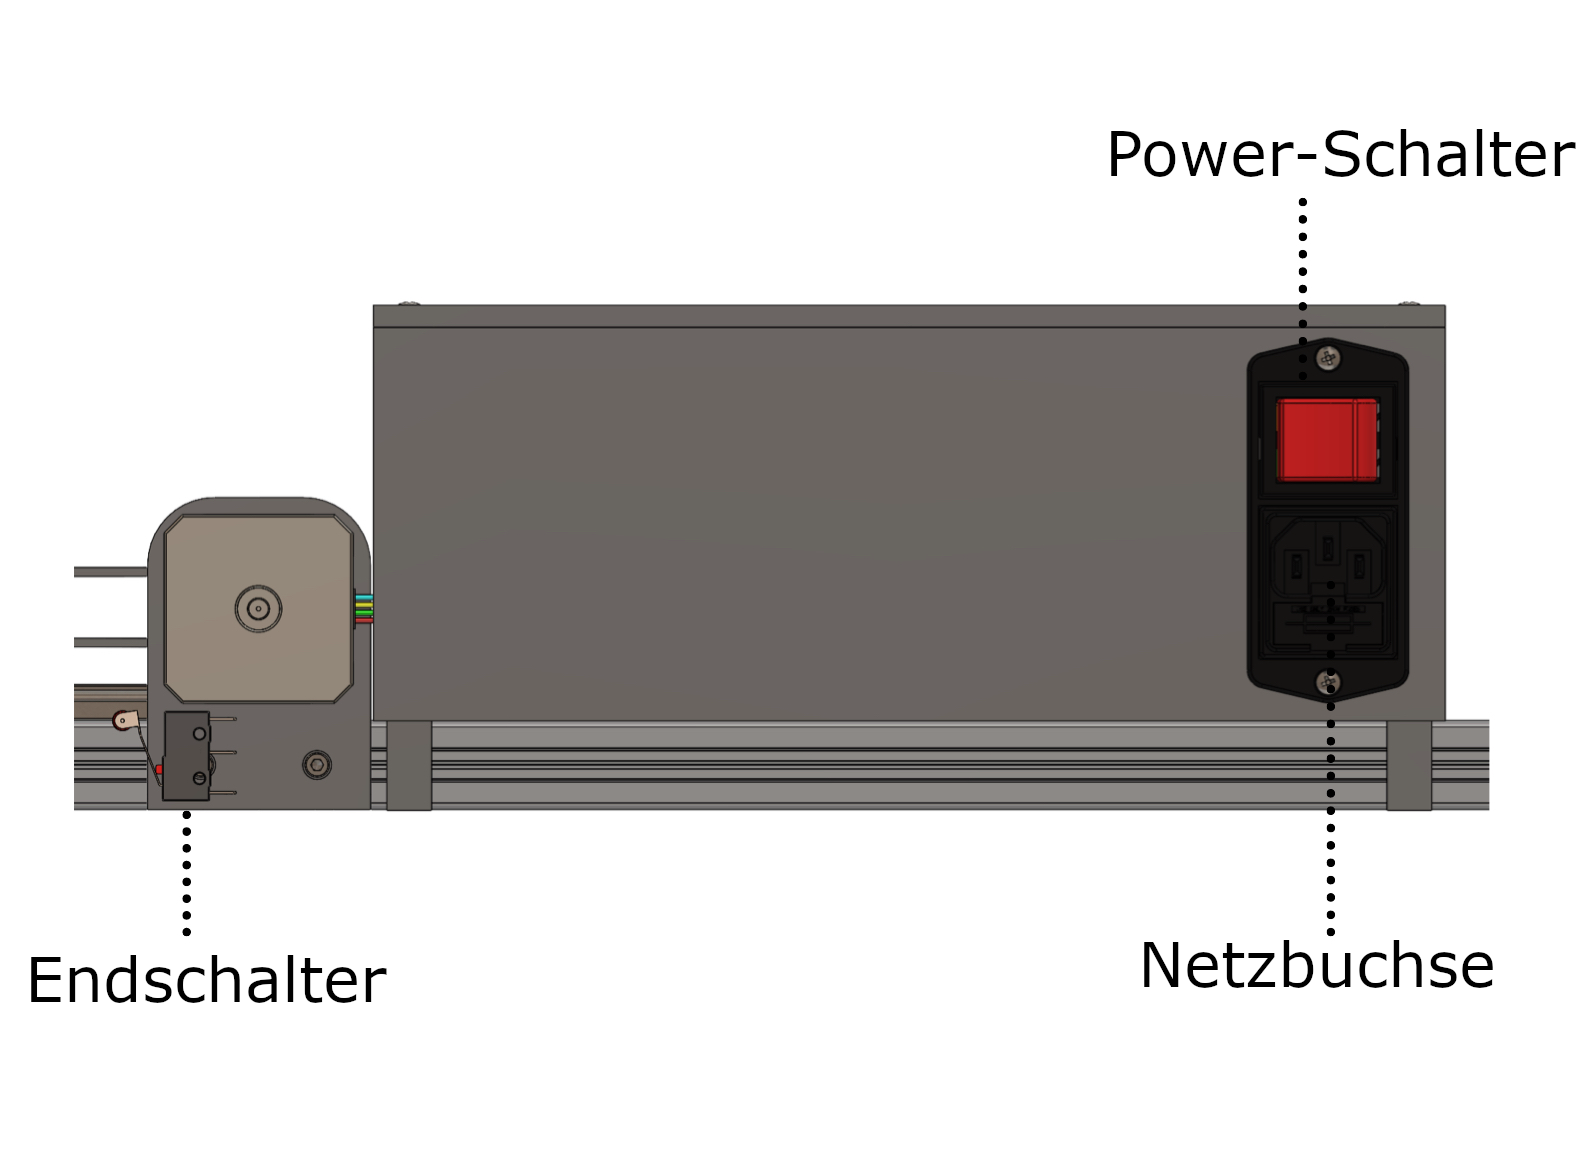
\includegraphics[width=\textwidth]{Images/Konstruktion3.png}
	%	\caption{Dies ist eine Konzeptskizze und wird noch ausgetauscht} \label{-}
\end{center}

\textbf{Power}: 
\begin{itemize}
	\item Ein- und ausschalten des Demonstrators
\end{itemize}

\textbf{Endschalter}: 
\begin{itemize}
	\item Zur Positionserfassung für die Referenzfahrt
\end{itemize}

\textbf{Netzkabel}: 
\begin{itemize}
	\item 1,8\ m langes Netzkabel zur Stromversorgung
\end{itemize}
